\section{Precessione}
    \begin{frame}
        \frametitle{Contenuti}
        \transblindsvertical
        \tableofcontents[currentsection]
    \end{frame}
    
    \begin{frame}{Calcolo della precessione}
        \begin{columns}
            \column{.5\textwidth}
                \begin{enumerate}
                    \item Individuazione perielio
                    \item Calcolare angolo con la posizione precedente del perielio - otteniamo $\frac{angolo}{periodo\ orbitale}$
                    \item Iterare il procedimento
                    \item Calcolare media e deviazione standard
                    \item Convertire in $\frac{arcsec}{anno\ terrestre}$ per confrontare coi adti reali
                \end{enumerate}
            \column{.5\textwidth}
                \centering
                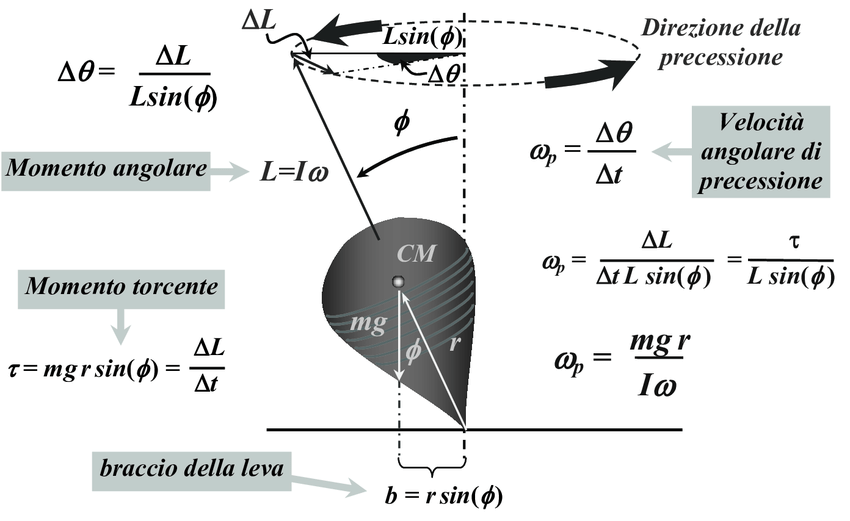
\includegraphics[width=.9\textwidth]{9_prec/precessione.png} \\
                \vspace{3mm}
                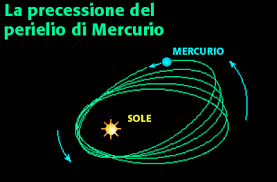
\includegraphics[width=.9\textwidth]{9_prec/mercurio.png}
        \end{columns}
    \end{frame}

    \begin{frame}{Modifiche al codice}
        \begin{block}{}
        \begin{enumerate}
            \item File di configurazione - aggiunta periodi rivoluzione pianeti
            \item classe Corpo Celeste  -
            \begin{enumerate}[a]
                \item Aggiunta membri m\_TT e m\_peri
                \item Modifiche a evolvidT()
                \item Correzione relativistica al calcolo dell'accelerazione
                \item Aggiunta funzione precessione() per l'analisi dei dati
                \item Aggiunta altri membri e metodi di servizio 
            \end{enumerate}
        \end{enumerate}
        \end{block}
        \begin{equation}
            \vec{a_i} = -\sum_{i\neq j}\frac{Gm_j}{r_{ij}^2}(1+\beta\frac{r_L^2}{r_{ij}^2})\frac{\vec r_{ij}}{r_{ij}}\,\,\,\,\,\,\,\,\forall i=1,\dots N
        \end{equation}
        \centering
        Con $\beta=3$ e $\vec{r_L}=\frac{\vec{L}}{mc}=\frac{\vec{r_{ij}}\times\vec{v_j}}{c}$
        %\begin{lstlisting}[language=C++]
void corpo::precessione(float Tterra){
    if(m_nome=="Sole")m_histos[7]->Fill(0);
    else{
        for(int i=1; i<m_peri.size(); i++){
            m_histos[7]->Fill
                (m_peri[i].angolo(m_peri[i-1])
                    *Tterra/m_TT);
        }
    }
}
\end{lstlisting}            
    \end{frame}

    \begin{frame}{Modifiche a corpo::evolvidT( ... ) - v1}
        \begin{lstlisting}[language=C++]
    [...]
    corpo sole*=cc[0];
    vettore sp=sole->P();
    float dSole=(m_pos-sp).modulo();
    [...]
    if(m_nome!="Sole"){
        float d_cfr=(m_app-m_sap).modulo();
        if(dSole<d_cfr){
            m_app=m_pos;
    	m_sap=sp;
        }
        uint64_t Tstep = m_TT *24*3600 / dt ;
        if((j+1)%Tstep == 0){
    	m_peri.push_back(m_app-m_sap);
    	m_app=m_pos;
    	m_sap=sp;
        }
    }
\end{lstlisting}
    \end{frame}
    \begin{frame}{Modifiche a corpo::evolvidT( ... ) - v2}
        \begin{lstlisting}[language=C++]
    corpo sole*=cc[0];
    if(m_nome=="Sole" && j<2){
	m_app=vettore(0,0,0);
    }
    else{
	m_app=m_pos0;
	m_sap=m_s0;
    }	
    m_s0=sole->P0();
    m_pos0=m_pos; [...]
    vettore sp=sole->P();
    float dSole=(m_pos-sp).modulo();
    if(m_nome!="Sole"){
	float d_media=(m_pos0-m_s0).modulo();
	float d_pre=(m_app-m_sap).modulo();
	if(d_media<d_pre && d_media<dSole)
		m_peri.push_back(m_pos0-m_s0);
    }
\end{lstlisting}
    \end{frame}

    \begin{frame}{Risultati (Obiettivo $= 56 \frac{arcsec}{anno\ terrestre}$)}
        Forte disaccordo coi dati reali:
        \vspace{3mm}
        \begin{columns}
            \column{.4\textwidth}
                \centering
                Senza Relatività
                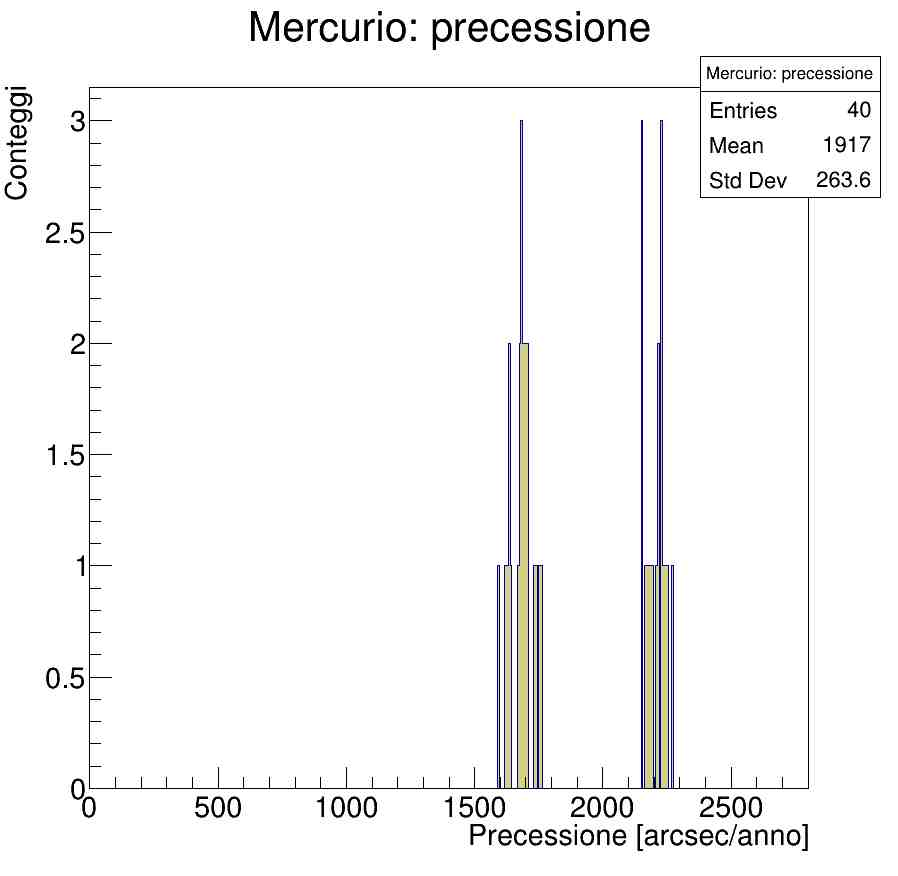
\includegraphics[width=\textwidth, height=3cm]{9_prec/sballati/10_3600_nor_1.jpg}\\
                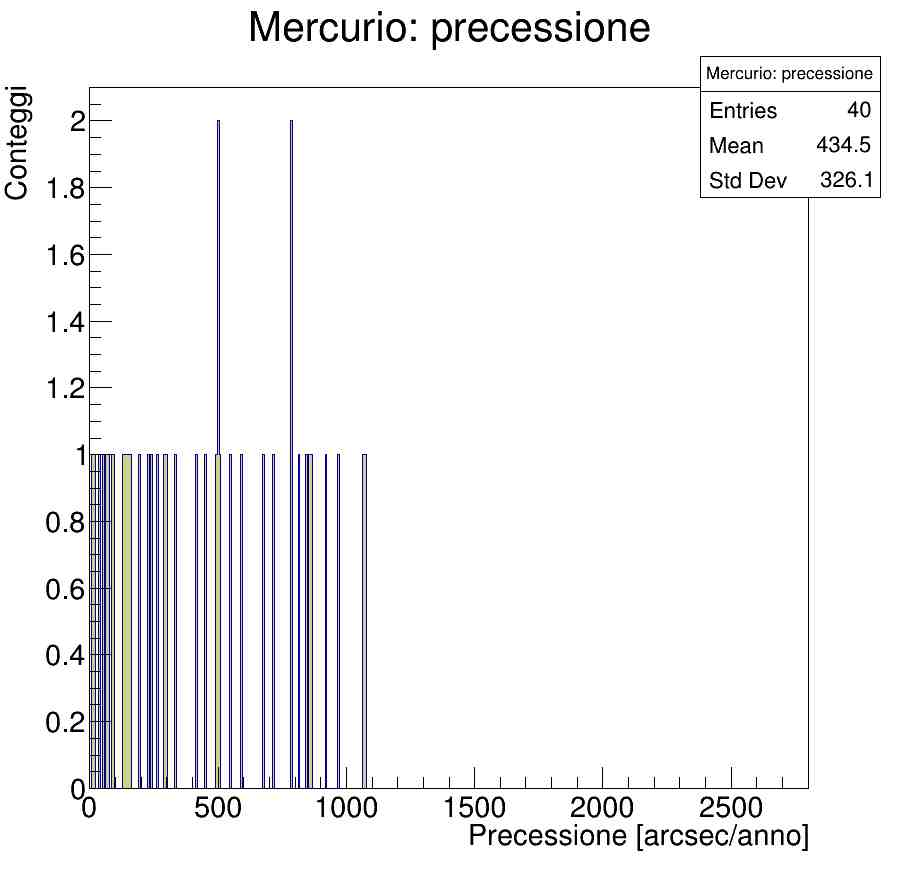
\includegraphics[width=\textwidth, height=3cm]{9_prec/sballati/10_60_nor_1.jpg}
            \column{.2\textwidth}
                \centering
                10a/3600s\\
                \vspace{3cm}
                10a/60s
            \column{.4\textwidth}
                \centering
                Con Relatività
                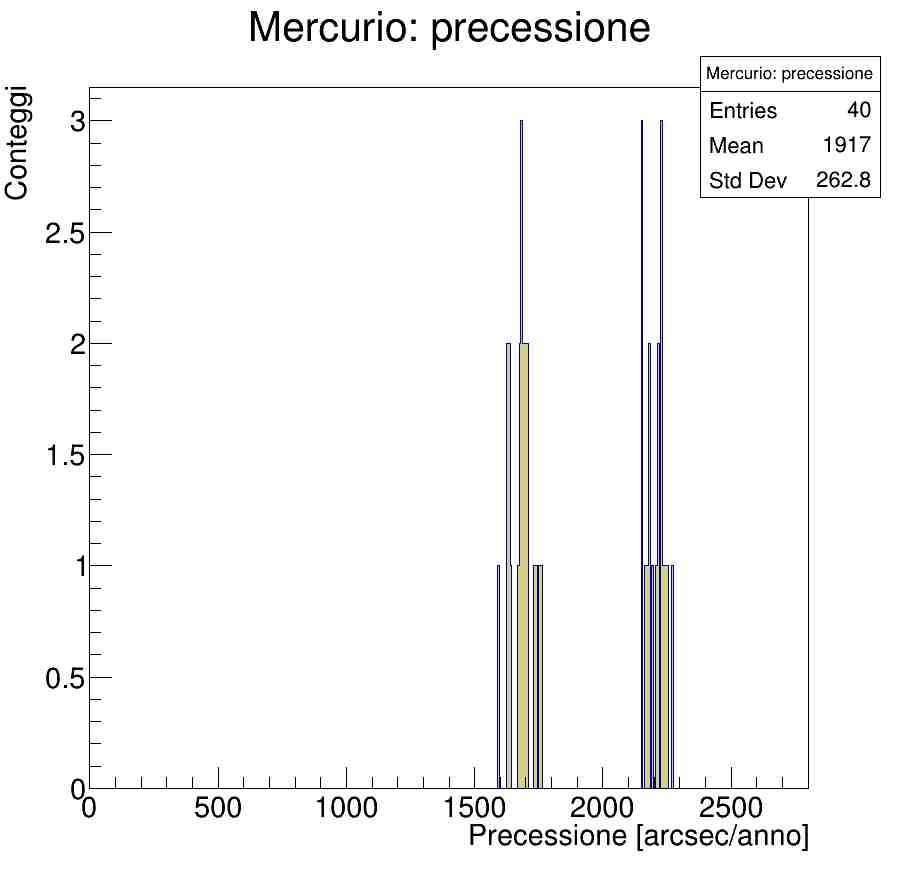
\includegraphics[width=.9\textwidth, height=3cm]{9_prec/sballati/10_3600_rel_1.jpg}\\
                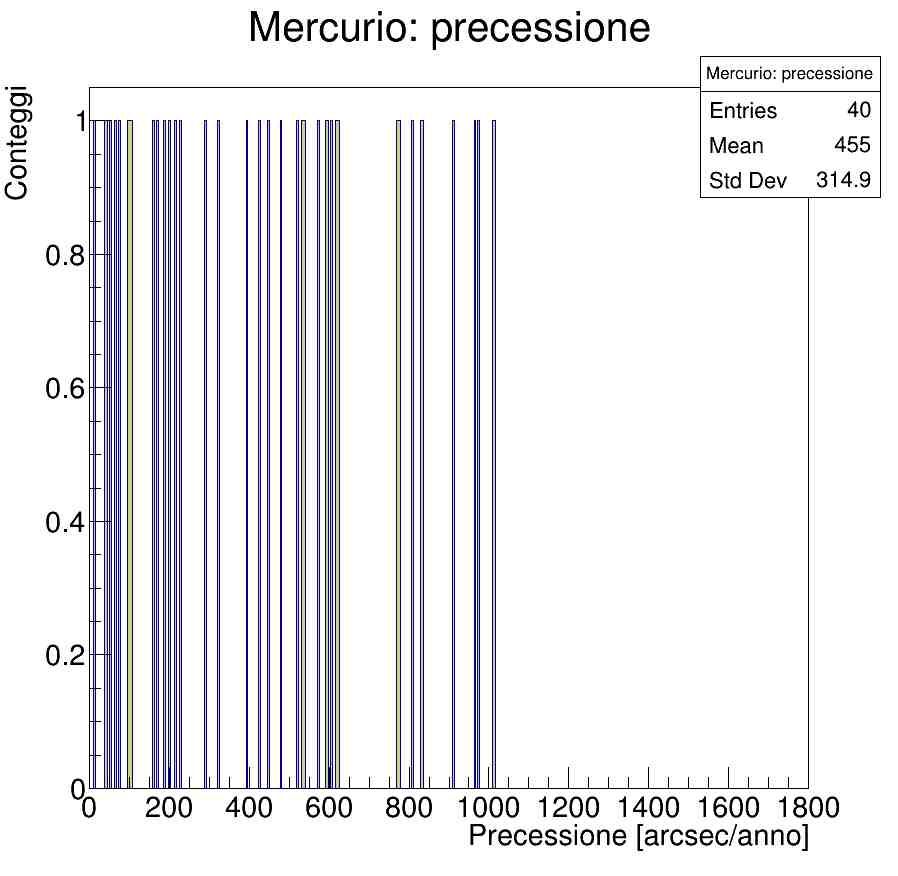
\includegraphics[width=.9\textwidth, height=3cm]{9_prec/sballati/10_60_rel_1.jpg}
        \end{columns}
    \end{frame}
    \begin{frame}{Risultati (Obiettivo $= 56 \frac{arcsec}{anno\ terrestre}$)}
        \begin{columns}
            \column{.4\textwidth}
                \centering
                Senza Relatività
                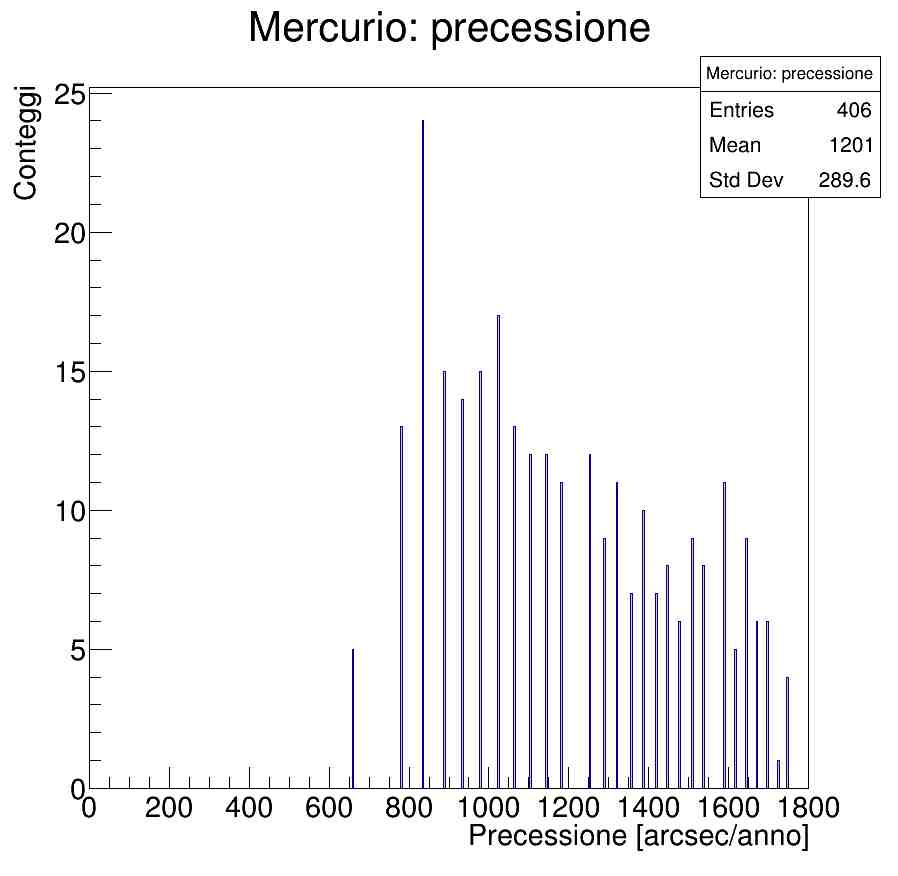
\includegraphics[width=\textwidth, height=3.25cm]{9_prec/sballati/100_3600_nor_1.jpg}\\
                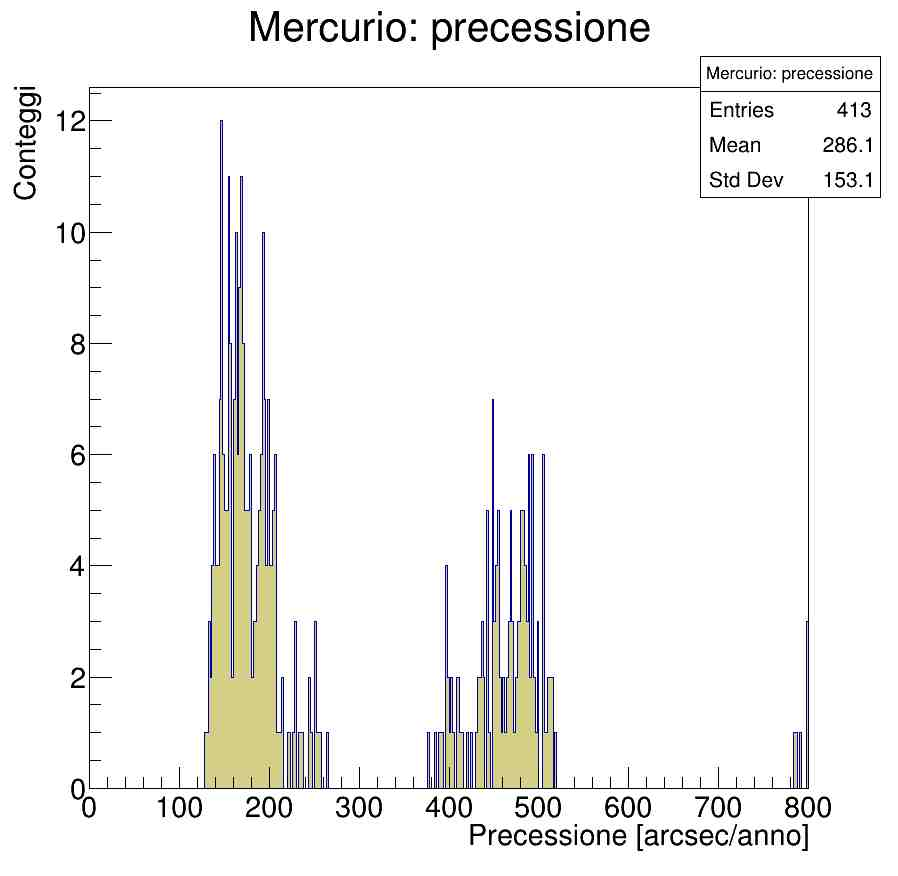
\includegraphics[width=\textwidth, height=3.25cm]{9_prec/sballati/100_600_nor_1.jpg}
            \column{.2\textwidth}
                \centering
                100a/3600s\\
                \vspace{3cm}
                100a/600s
            \column{.4\textwidth}
                \centering
                Con Relatività
                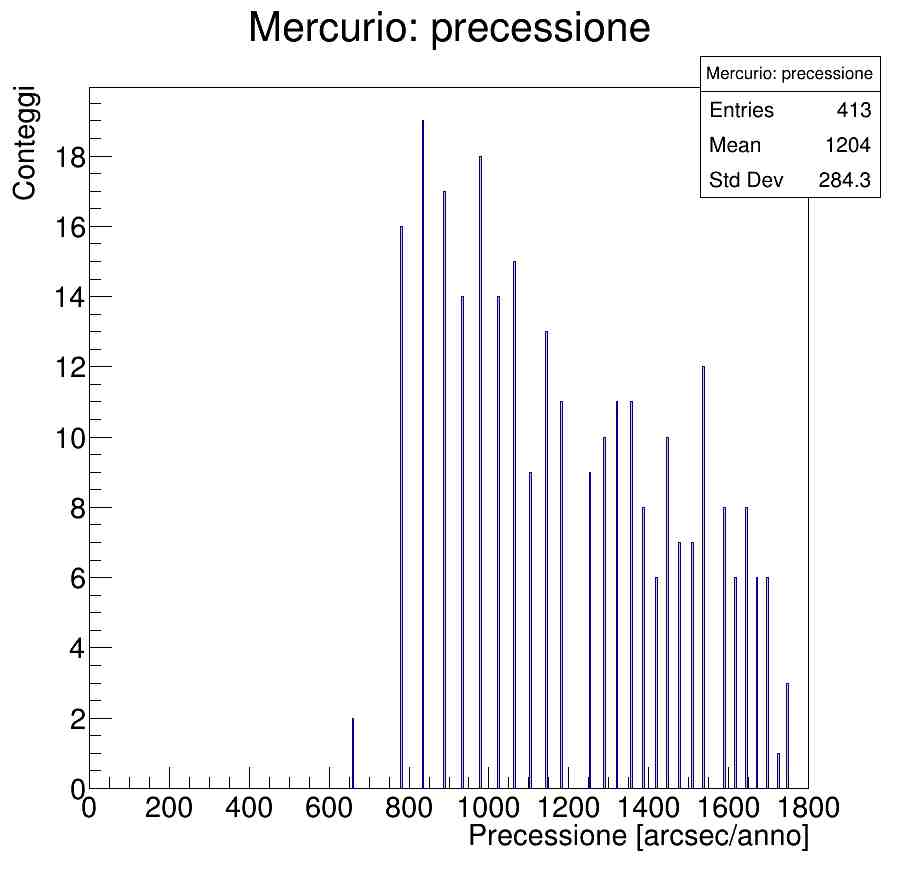
\includegraphics[width=\textwidth, height=3.25cm]{9_prec/sballati/100_3600_rel_1.jpg}\\
                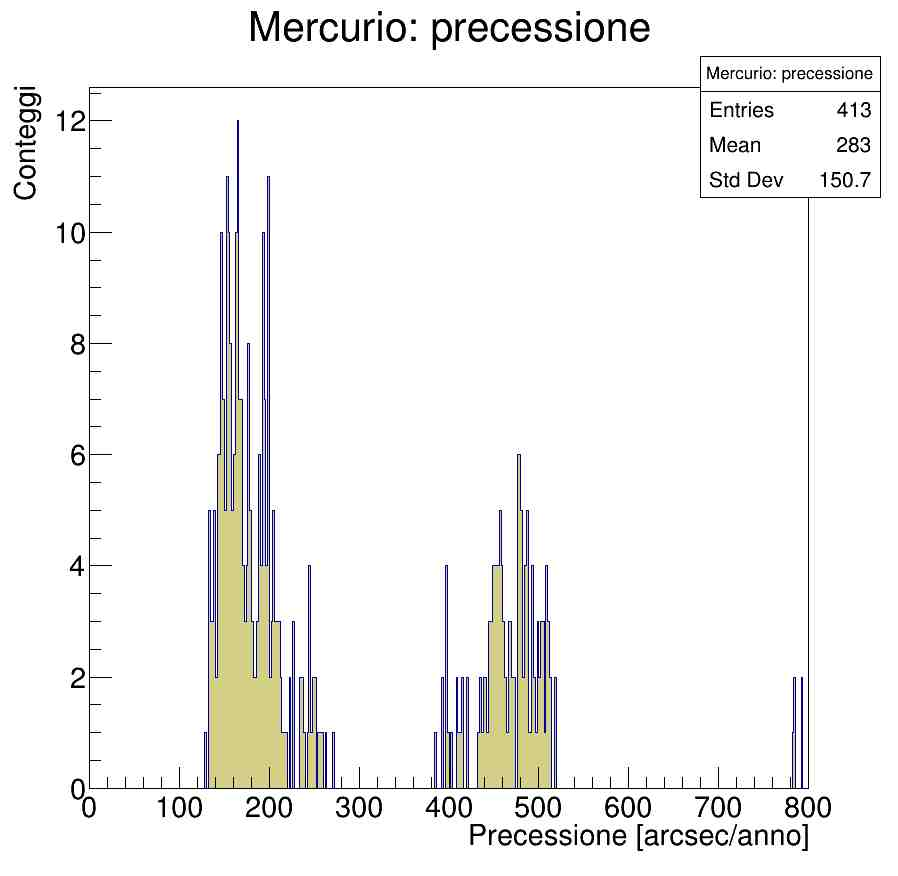
\includegraphics[width=\textwidth, height=3.25cm]{9_prec/sballati/100_600_rel_1.jpg}
        \end{columns}
    \end{frame}
    \begin{frame}{Risultati (Obiettivo $= 56 \frac{arcsec}{anno\ terrestre}$)}
        \begin{columns}
            \column{.4\textwidth}
                \centering
                Senza Relatività
                \includegraphics[width=\textwidth, height=3.25cm]{9_prec/sballati/10_6_nor_1.jpg}\\
                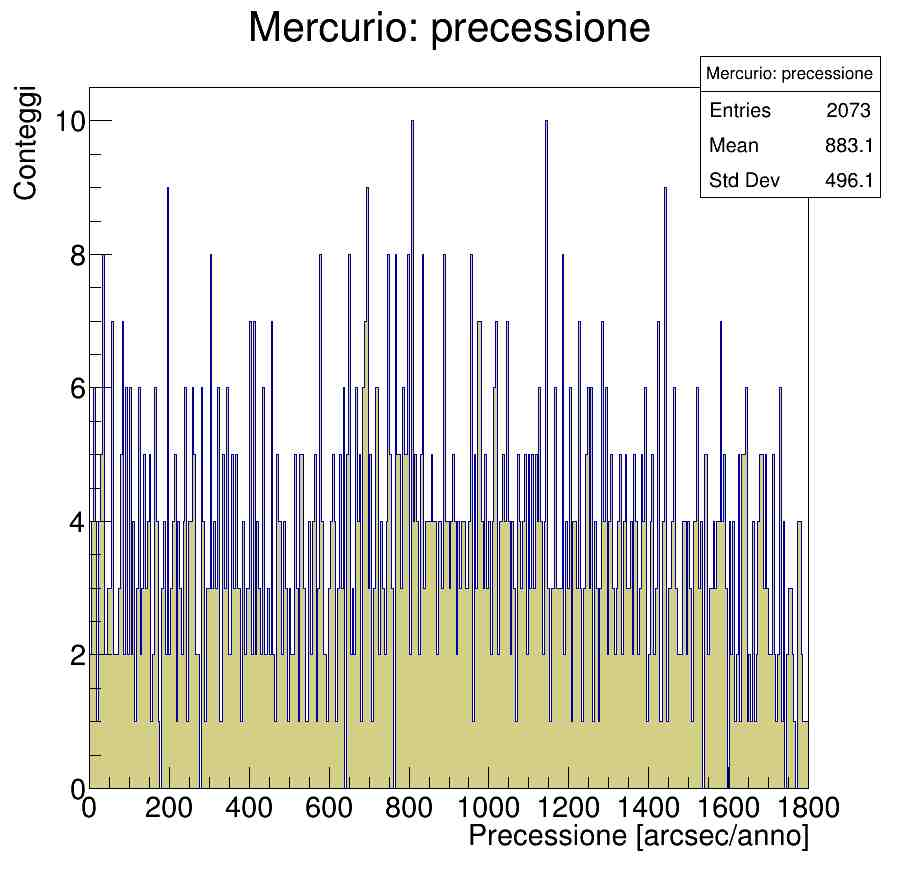
\includegraphics[width=\textwidth, height=3.25cm]{9_prec/sballati/500_3600_nor_1.jpg}
            \column{.2\textwidth}
                \centering
                10a/6s
                \vspace{3cm}
                500a/3600s
            \column{.4\textwidth}
                \centering
                Con Relatività
                \includegraphics[width=\textwidth, height=3.25cm]{9_prec/sballati/10_6_rel_1.jpg}\\
                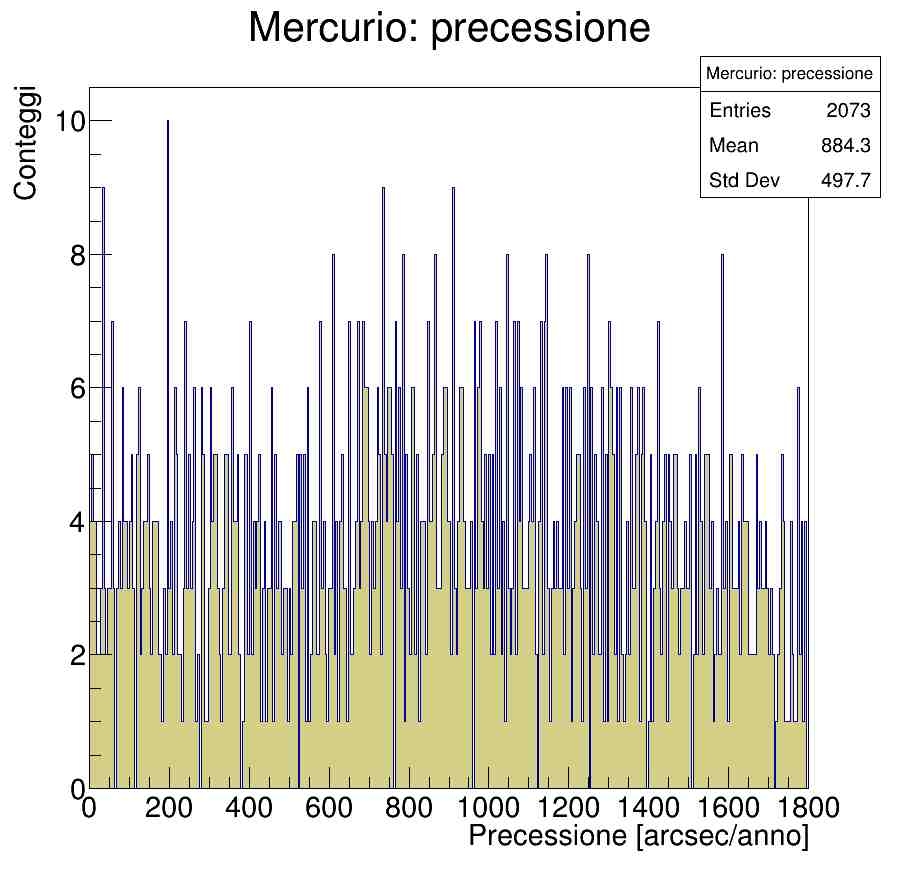
\includegraphics[width=\textwidth, height=3.25cm]{9_prec/sballati/500_3600_rel_1.jpg}
        \end{columns}
    \end{frame}

    \begin{frame}{Risultati (Obiettivo $= 56 \frac{arcsec}{anno\ terrestre}$)}
        \begin{columns}
            \column{.4\textwidth}
                \centering
                Con Relatività solo rispetto al sole
                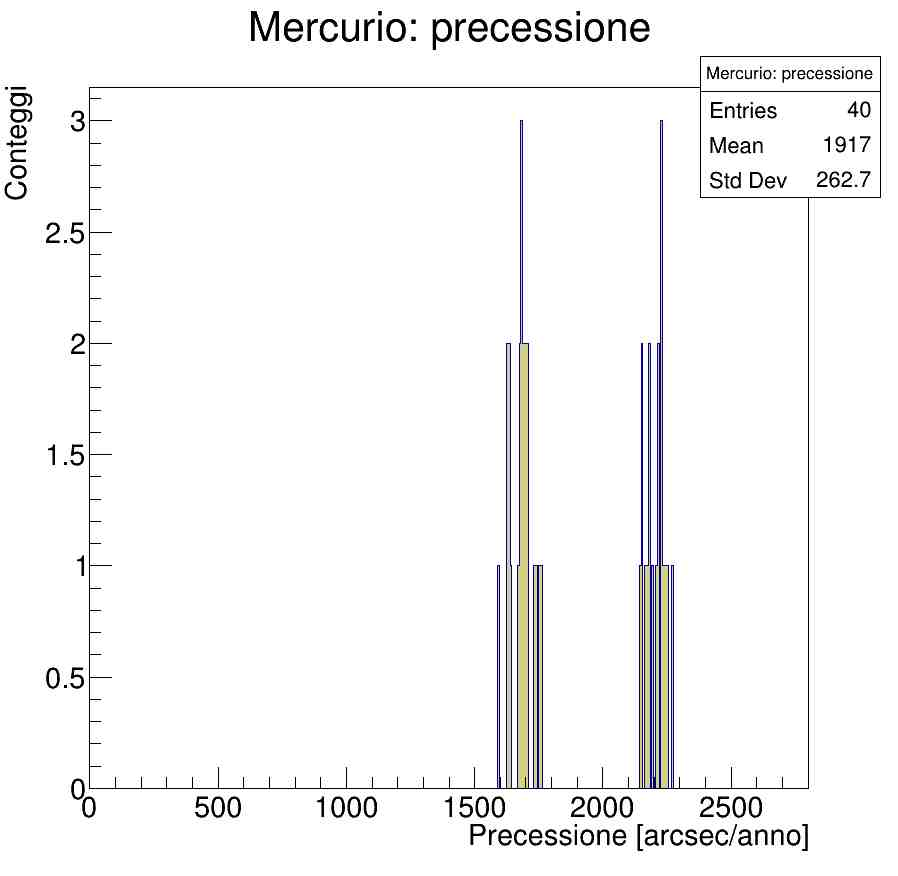
\includegraphics[width=\textwidth, height=3.25cm]{9_prec/sballati/10_3600_relB_1.jpg}\\
                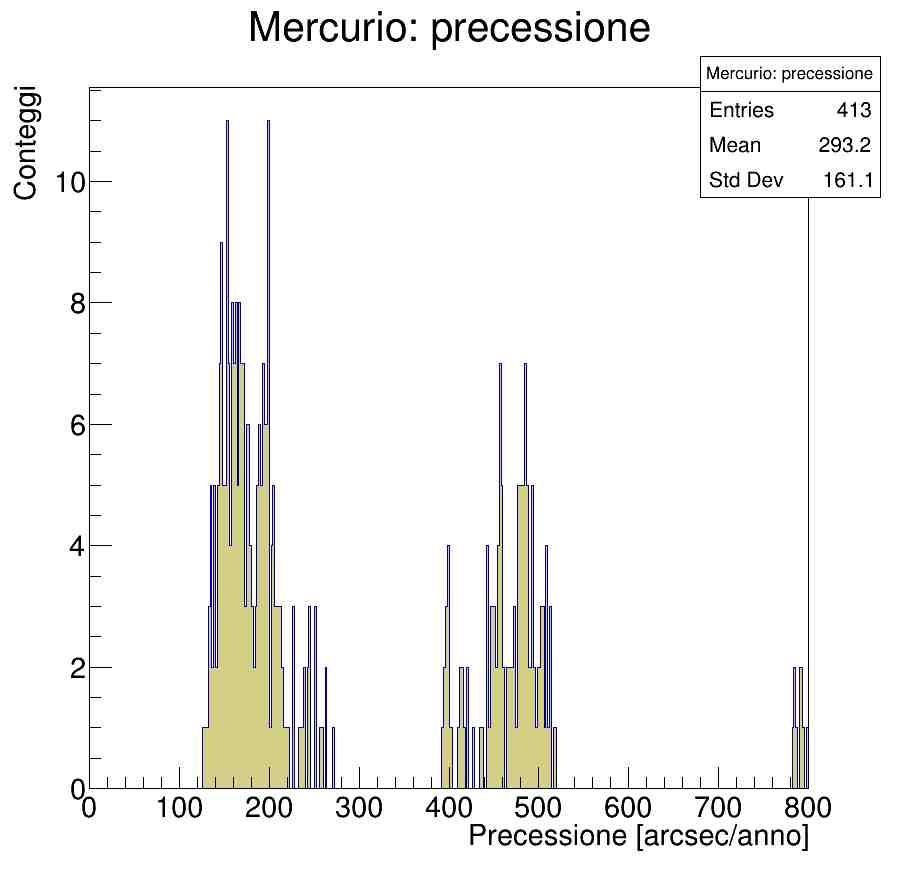
\includegraphics[width=\textwidth, height=3.25cm]{9_prec/sballati/100_600_relB_1.jpg}
            \column{.2\textwidth}
                \centering
                10a/3600s\\
                \vspace{3cm}
                100a/600s
            \column{.4\textwidth}
                \centering
                Con Relatività
                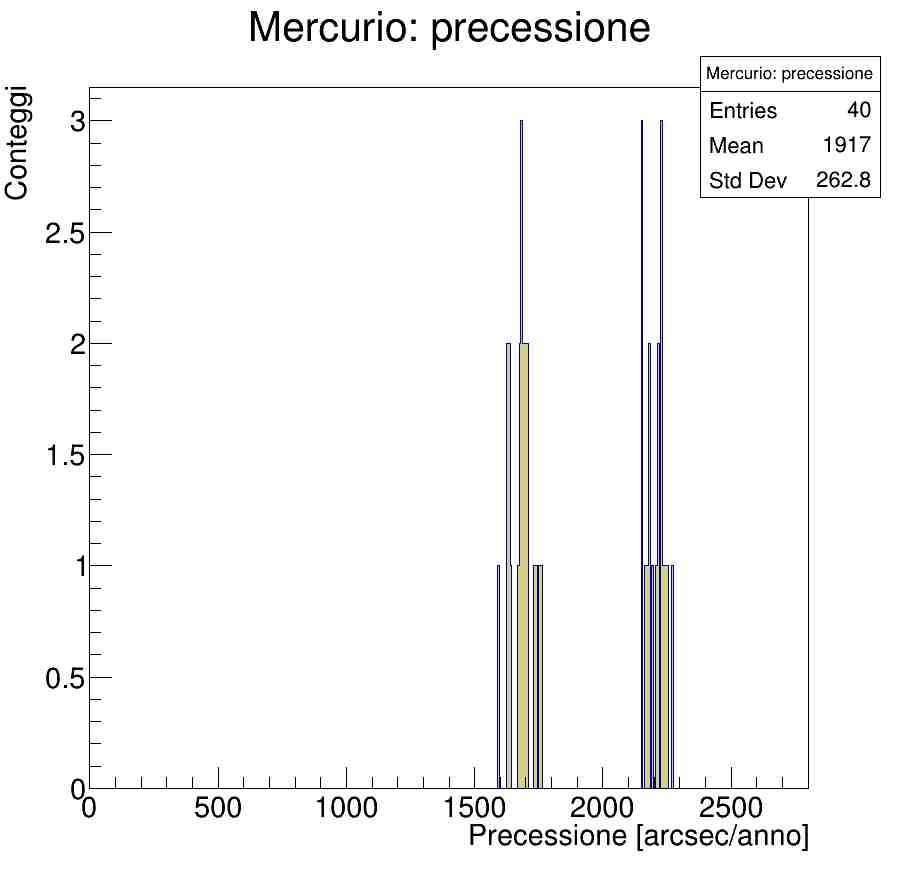
\includegraphics[width=\textwidth, height=3.25cm]{9_prec/sballati/10_3600_rel_1.jpg}\\
                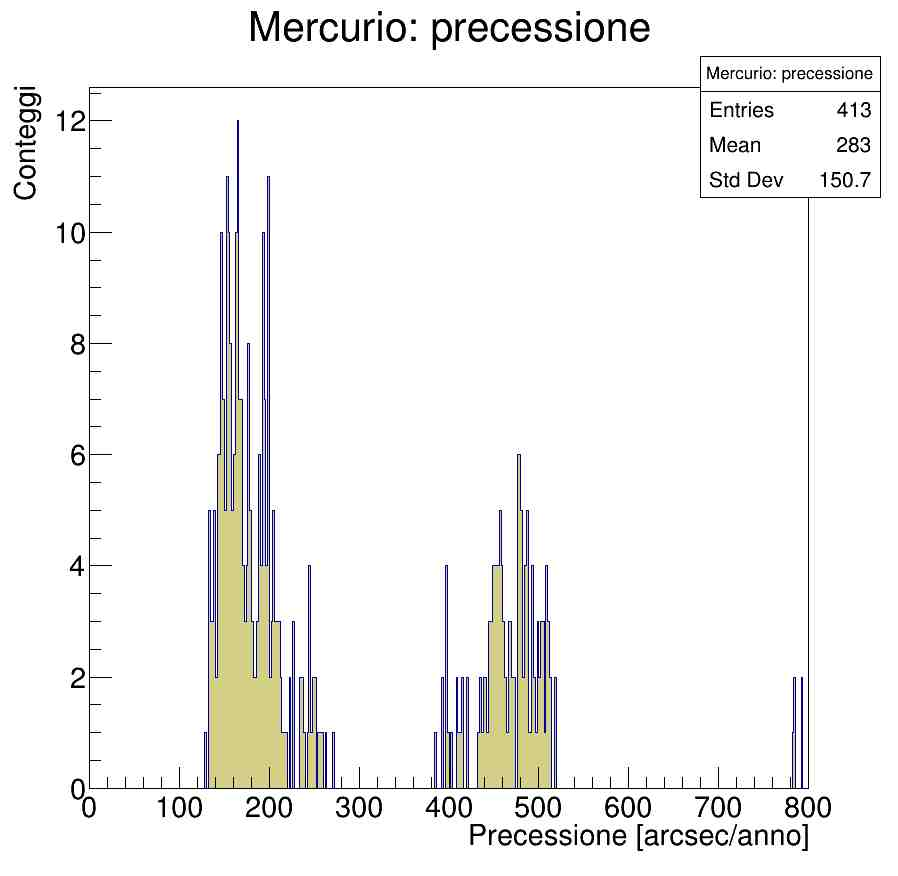
\includegraphics[width=\textwidth, height=3.25cm]{9_prec/sballati/100_600_rel_1.jpg}
        \end{columns}
    \end{frame}